%=============================================================================
% SECTION 2 - Steps in MUSIC Algorithm
%=============================================================================

\section{Teoria din spatele algoritmului MUSIC}
\label{sec:theory-music}

\begin{figure}[h]
    \centering
    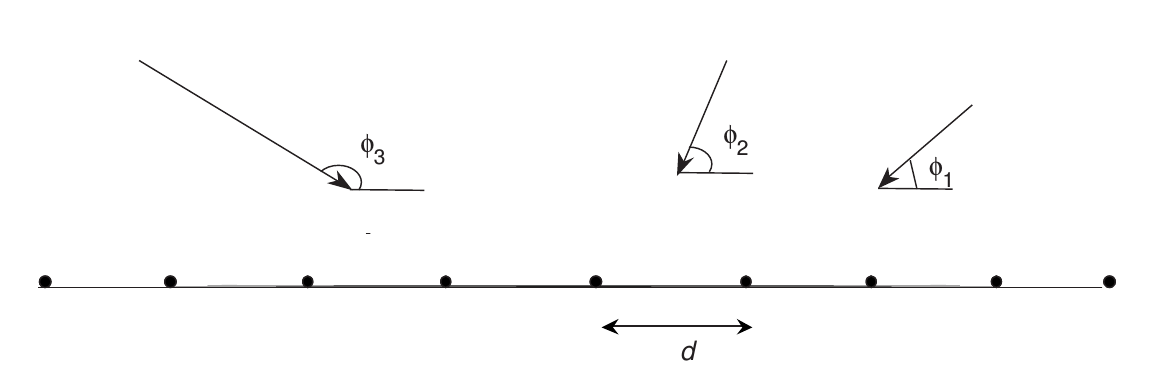
\includegraphics[width=1\textwidth]{array-for-doa}
    \caption{TODO: my own image in PS}
    \label{fig:array-for-doa}
\end{figure}


În analiza algoritmului MUSIC presupunem că plecăm de la un șir liniar de $M$
antene la care ajung $D$ semnale $s_j(t), i = \overline{1, D}$ și se dorește
estimarea unghiului de incidență $\theta_j$ măsurat față de axa $x$ în sens
trigonometric sub care ajunge fiecare semnal la șirul de antene. Presupunem că
mediul de propagare nu afectează semnificativ semnalele când acestea se propagă
de la un element din șir la altul, deci semnalul care ajunge la o antenă diferă
de cel care ajunge la o altă antenă doar printr-o întârziere $\tau$. \\

Considerăm că prima antenă se află în originea sistemului, la locația (0, 0) și
exprimăm întarzierea semnalului de la celelalte elemente din șir relativ la
semnalul care ajunge la elementul de referință. Astfel, pentru un șir liniar,
semnalul $j$ care ajunge la elementul $i = 2$ parcurge o distanță mai lungă cu
$d\,cos\theta_j$ față de primul element și, în cazul general, putem scrie
întârzierea $\tau_i$ la elementul $i$ ca
\begin{equation}
    \tau_i = \beta(i-1)d\,cos\theta_j
\end{equation}
unde $\beta = \frac{2\pi}{\lambda}$ este factorul de defazaj. \\

Aici, am presupus că defazajul semnalului depinde doar de locațiile distincte
ale elementelor șirului de antene. În realitate, antenele vor avea și ele un
răspuns dependent de directivitatea lor și de frecvență, care poate fi modelat
ca un câștig $g_i$. Obținem, astfel, vectorul director (\textit{steering
vector}) pentru un anumit unghi de incidență $\theta_j$ și frecvență $\omega$:
\begin{equation}
    \bm{a}(\omega, \theta_j) = 
	    \begin{bmatrix}
		g_1(\omega, \theta_j)e^{\tau_1(\theta_j)} \\
		... \\
		g_M(\omega, \theta_j)e^{\tau_M(\theta_j)}
	    \end{bmatrix}
\end{equation}

Prin urmare, vectorul director este dependent de răspunsul individual al
fiecărui element din șirul de antene, de geometria șirului, de frecvența
semnalului și de unghiul de incidență al acestuia. Matricea care se formează din
vectorii coloană directori pentru toate unghiurile de incidență și toate
frecvențele se numește matricea colectoare a șirului
(\textit{array manifold matrix}).
\begin{equation}
    \bm{A} = 
	    \begin{bmatrix}
		\bm{a}(\omega, \theta_1) & ... & \bm{a}(\omega, \theta_D)
	    \end{bmatrix}
\end{equation}

Dacă banda semnalului este suficient de îngustă, se poate considera, cu
aproximație, că vectorul director este independent de frecvență și că depinde doar
de unghiul de incidență. Mai mult, dacă presupunem că elementele șirului sunt
izotrope, putem elimina dependența vectorului director de câștigul $g_i,
i = \overline{1, M}$. Vom continua analiza având în vedere aceste presupuneri.\\

Putem scrie următoarea relație pentru semnalele de la intrarea fiecărei antene
din șir:
\begin{equation}
\label{eq:xasn}    
    \bm{x}(t) = 
	\begin{bmatrix}
	   \bm{a}(\theta_1) & \bm{a}(\theta_2) & ... & \bm{a}(\theta_D)
	\end{bmatrix}
	\begin{bmatrix}
	    s_1(t) \\ s_2(t) \\ ... \\ s_D(t)
	\end{bmatrix}
	+
	\begin{bmatrix}
	    n_1(t) \\ n_2(t) \\ ... \\ n_D(t)
	\end{bmatrix}
\end{equation}
\begin{equation}
\label{eq:xasn-short}
    \bm{x}(t) = \bm{A}\bm{s}(t) + \bm{n}(t)
\end{equation}

% (TODO: puțin despre cine l-a făcut + citează \cite{cite:music-schmidt})
Algoritmul MUSIC (MUltiple SIgnal Classification) face parte dintr-o clasă mai
mare de algoritmi care se bazează pe metoda subspațiilor, care ia în considerare
și zgomotul dintr-un sistem. Algoritmul oferă, în primul rând, informații despre
numărul de semnale care ajung la un șir de antene și unghiul de incidență al
acestora. Este un algoritm cu rezoluție mare, ceea ce înseamnă că poate distinge
mai ușor decât alți algoritmi două semnale care vin din direcții foarte
apropiate, dar are nevoie de o calibrare foarte precisă a șirului de antene.
Calibrarea constă în obținerea matricei colectoare a șirului de antene; în
practică, acest lucru se realizează măsurând răspunsurilor unor surse
punctiforme ale șirului la diverse unghiuri și frecvențe. Pentru explicarea
fundamentului matematic din spatele algoritmului MUSIC s-a folosit ca referință
lucrarea \cite{cite:doa-1996}, în care este tratat pe larg subiectul estimării
unghiurilor de incidență folosind șiruri de antene.\\

În ecuația \eqref{eq:xasn}, vectorul $\bm{x}$ al semnalelor de la intrarea
antenelor din șir și vectorii directori $\bm{a}(\theta_j), j = \overline{1, D}$
pot fi priviți ca vectori într-un spațiu cu M dimensiuni, ceea ce înseamnă că
$\bm{x}$ poate fi scris ca o combinație liniară între vectorii directori, unde $s_j,
j = \overline{1, D}$ sunt coeficienții combinațiilor. \\

Se poate calcula matricea de covarianță a intrării
\begin{equation}
    \bm{R}_{xx} = E[\bm{xx}^H] = \bm{A}E[\bm{ss}^H]\bm{A}^H + E[\bm{nn}^H]
\end{equation}
\begin{equation}
    \bm{R}_{xx} = \bm{A}\bm{R}_{ss}\bm{A}^H + \sigma^2_{zg}\bm{I}
\end{equation}

S-a notat $\bm{R}_{ss} = E[\bm{ss}^H]$ matricea de corelație a semnalului $s$.
Se observă două proprietăți importante:
\begin{itemize}
    \item Vectorii directori sunt liniar independenți, ceea ce înseamnă că
    matricea $\bm{A}$ este de rang maxim.
    \item $\bm{R}_{ss}$ este o matrice nesingulară dacă semnalele incidente sunt
    cel mult parțial necorelate. Dacă ar fi corelate, atunci cel puțin una
    dintre liniile/coloanele sale ar putea fi scrisă ca o combinație liniară a
    altor linii/coloane, ceea ce ar însemna că matricea ar avea determinantul
    egal cu 0, deci ar fi singulară și nu am mai putea folosi algoritmul.
\end{itemize}

Din aceste două proprietăți rezultă că, dacă $M < D$, atunci matricea
$\bm{A}\bm{R}_{ss}\bm{A}^H$ este pozitiv semidefinită, având rangul D. Din
această proprietate, se poate demonstra faptul că $M - D$ dintre valorile
proprii ale matricei trebuie să fie nule. Folosind relația
\eqref{eq:xasn-short}, reiese că atunci când $M - D$ dintre valorile proprii ale
matricei $\bm{A}\bm{R}_{ss}\bm{A}^H$ sunt nule, cele mai mici valori proprii ale
matricei $\bm{R}_{xx}$ vor fi egale cu puterea zgomotului $\sigma_{zg}^2$. Dacă
notăm $\lambda_i, i = \overline{1, M}$ valorile proprii ale matricei
$\bm{R}_{xx}$, atunci
\begin{equation}
    \lambda_{D+1} = \lambda_{D+2} = ... = \lambda_M = \lambda_{min} = \sigma_{zg}^2
\end{equation}

În realitate, însă, nu se va îndeplini egalitatea, deoarece folosim
pentru estimare doar un număr finit de eșantioane, dar valorile vor fi,
într-adevăr, foarte apropiate. Dacă notăm $K$ multiplicitatea celei mai mici
valori proprii a matricei $\bm{R}_{xx}$, atunci, știind că $M = D + K$, putem
estima numărul semnalelor care ajung la șirul de antene
\begin{equation}
    \hat{D} = M - K
\end{equation}

Din definițiile valorilor proprii și a vectorilor proprii \cite{cite:gol-89}, vectorii
proprii $\bm{v}_i, i = \overline{1, M}$ corespunzători celor mai mici valori
proprii trebuie să satisfacă egalitatea
\begin{equation}
    \bm{R}_{xx}\bm{v}_i = \sigma_{zg}^2\bm{v}_i, \quad i = \overline{D+1, M}
\end{equation}
Folosind ecuația \eqref{eq:xasn-short}, înseamnă că
\begin{equation}
    \bm{A}\bm{R}_{ss}\bm{A}^H\bm{v}_i = 0, \quad i = \overline{D+1, M}
\end{equation}
Știind că $\bm{A}$ este de rang maxim și că $\bm{R}_{ss}$ este nesingulară,
atunci
\begin{equation}
    \bm{A}^H\bm{v}_i = 0, \quad i = \overline{D+1, M}
\end{equation}
ceea ce este echivalent cu a spune că vectorii coloană ai matricei $\bm{A}$,
adică vectorii directori, sunt perpendiculari pe vectorii proprii ai matricei
$\bm{R}_{xx}$. 
\begin{equation}
    \begin{bmatrix}
	\bm{a}(\theta_1) & \bm{a}(\theta_2) & ... & \bm{a}(\theta_D)
    \end{bmatrix}
    \bot
    \begin{bmatrix}
	\bm{v}_{D+1} & \bm{v}_{D+2} & ... & \bm{v}_M
    \end{bmatrix}
\end{equation}

Recapitulând, avem două subspații ortogonale: cel al semnalelor și cel al
zgomotului. Vectorii directori ai șirului de antene aparțin subspațiului
semnalelor și, așadar, sunt perpendiculari pe subspațiul zgomotului, iar
vectorii proprii ai matricei de covarianță $\bm{R}_{xx}$ pot aparține oricăruia
dintre cele două subspații. Prin urmare, putem să căutăm printre vectorii
directori pe aceia care sunt ortogonali pe subspațiul zgomotului, în care se vor
afla o parte din vectorii proprii ai matricei de covarianță, și să determinăm
unghiurile de incidență $\theta_j$.

Se calculează spectrul MUSIC folosind una dintre următoarele două forumle:
\begin{equation}
    P_{MUSIC}(\theta) =
        \frac{\bm{a}^H(\theta)\bm{a}(\theta)}
             {\bm{a}^H(\theta)\bm{V}_N\bm{V}_N^H\bm{a}(\theta)} \\
\end{equation}
\begin{equation}
    P_{MUSIC}(\theta) =
        \frac{1}
             {\bm{a}^H(\theta)\bm{V}_N\bm{V}_N^H\bm{a}(\theta)} \\
\label{eq:music-spectrum}
\end{equation}
\begin{equation}
    \bm{V}_N = \begin{bmatrix}v_{D+1}, & ..., & v_M \end{bmatrix}
\end{equation}
și, în cazul în care vectorii directori sunt perpendiculari pe vectorii proprii,
numitorul va fi minim, ceea ce va conduce la apariția unor vârfuri în spectru.
Cunoaștem numărul de semnale estimat $\hat{D}$, deci cele $\hat{D}$
vârfuri din spectru corespund unghiurilor de incidență căutate.
